% -----------------------------------------------
% Template for ISMIR Papers
% 2019 version, based on previous ISMIR templates

% Requirements :
% * 6+n page length maximum
% * 4MB maximum file size
% * Copyright note must appear in the bottom left corner of first page
% * Clearer statement about citing own work in anonymized submission
% (see conference website for additional details)
% -----------------------------------------------

\documentclass{article}
\usepackage[T1]{fontenc} % add special characters (e.g., umlaute)
\usepackage[utf8]{inputenc} % set utf-8 as default input encoding
\usepackage{ismir,amsmath,cite,url}
\usepackage{graphicx}
\usepackage{color}

% Optional: To use hyperref, uncomment the following.
% \usepackage[bookmarks=false,hidelinks]{hyperref}
% Mind the bookmarks=false option; bookmarks are incompatible with ismir.sty.

\newcommand{\setNameUpper}{FOURIER}
\newcommand{\setName}{Fourier}

% Title.
% ------
\title{The \setNameUpper~Set: Beats, Downbeats, and Functional Segment Annotations of Western Popular Music}

% Note: Please do NOT use \thanks or a \footnote in any of the author markup

% Single address
% To use with only one author or several with the same address
% ---------------
%\oneauthor
% {Names should be omitted for double-blind reviewing}
% {Affiliations should be omitted for double-blind reviewing}

% Two addresses
% --------------
%\twoauthors
%  {First author} {School \\ Department}
%  {Second author} {Company \\ Address}

%% To make customize author list in Creative Common license, uncomment and customize the next line
%  \def\authorname{First Author, Second Author}


% Three addresses
% --------------
\threeauthors
  {First Author} {Affiliation1 \\ {\tt author1@ismir.edu}}
  {Second Author} {\bf Retain these fake authors in\\\bf submission to preserve the formatting}
  {Third Author} {Affiliation3 \\ {\tt author3@ismir.edu}}

%% To make customize author list in Creative Common license, uncomment and customize the next line
%  \def\authorname{First Author, Second Author, Third Author}

% Four or more addresses
% OR alternative format for large number of co-authors
% ------------
%\multauthor
%{First author$^1$ \hspace{1cm} Second author$^1$ \hspace{1cm} Third author$^2$} { \bfseries{Fourth author$^3$ \hspace{1cm} Fifth author$^2$ \hspace{1cm} Sixth author$^1$}\\
%  $^1$ Department of Computer Science, University , Country\\
%$^2$ International Laboratories, City, Country\\
%$^3$  Company, Address\\
%{\tt\small CorrespondenceAuthor@ismir.edu, PossibleOtherAuthor@ismir.edu}
%}
%\def\authorname{First author, Second author, Third author, Fourth author, Fifth author, Sixth author}


\sloppy % please retain sloppy command for improved formatting

\begin{document}

%
\maketitle
%
\begin{abstract}
    We introduce the \setName\footnote{Temporary name for the blind review process.}~set: a collection of annotations of beats, downbeats, and functional segmentation for over 700 tracks that covers a wide range of western popular music.
    Given the variety of annotated music information types in this set, and how strongly these three types of data are typically intertwined, we believe it could potentially foster research that focuses on multiple retrieval tasks at once.
    The dataset includes additional metadata such as MusicBrainz identifiers to support the linking of the dataset to third-party information or audio data when available.
    We describe the methodology employed in acquiring this set, including the annotation process and song selection. 
    In addition an initial data exploration of the annotations and actual dataset content is conducted. 
    Finally, we provide a series of baselines of the \setName~set with standard beat-trackers, downbeat predictors, and structural segmentation algorithms in the literature.
\end{abstract}
%
\section{Introduction}\label{sec:introduction}

The tasks of beat detection, downbeat prediction, and structural segmentation~\cite{Paulus2010} constitute a fundamental part of the field of MIR.
These three musical characteristics are often related: downbeats define the first beat of a given music measure, and long structural music segments tend to begin and end on specific beat locations --frequently on downbeats.
The automatic estimation of such information could result in better musical systems such as more accurate automatic DJ-ing, better intra- and inter-song navigation, further musicological insights of large collections, \emph{etc}.
While several approaches exploiting more than one of these musical traits have been proposed~\cite{Bock2016, Mccallum2019, Fuentes2019}, the lack of human annotated data containing the three of them for a single collection are scarce.
This limits the amount of potential of certain methods, especially those that require large amounts of information (e.g., deep learning~\cite{Humphrey2012}).

In this paper we present the \setName~set: human annotations of beats, downbeats, and functional segmentation for over 700 tracks of western popular music.
These annotations were gathered with the aim of having a significant amount of data to train models to improve the prediction of such musical attributes, which would later be applied to various products offered by the company \setName.
By releasing this set to the public, it is our aim to let the research community explore and exploit these annotations to advance the tasks of beat tracking, downbeat prediction, and automatic functional structural segmentation.
We discuss the methodology to acquire these data, including the song selection process, and the inclusion of standard identifiers (Acoustid and MusicBrainz) and onsets for the first 30 seconds of the tracks to allow for other researchers to more easily access and align, when needed, the actual audio content.
Furthermore, we present a series of results with standard algorithmic approaches in the literature with the goal of having an initial public benchmark of this set.

The rest of this work is organized as follows: Section~\ref{sec:background} contains a review of the most relevant public datasets of the tasks at hand; Section~\ref{sec:dataset} discusses the actual \setName~set, including the data gathering, their formatting, and various statistics; Section~\ref{sec:results} presents various benchmarks in the set; and Section~\ref{sec:conclusions} draws some final conclusions and discloses future remarks.
%
\section{Background}\label{sec:background}

In this section we discuss previously published datasets and the tasks they aim to solve.

% Introduce on beat annotation
\subsection{Beat and Downbeat Tracking Sets}

Over the last 15 years, many annotated datasets for beat and downbeat tracking have appeared in the literature whose primary purpose has been to allow the comparison of newly proposed and existing algorithms. However, the well-known difficulties of sharing the audio component of large annotated datasets has led to a rather ad-hoc usage of different datasets within the literature, and to a lesser extent, the choice of which evaluation metrics are selected to report accuracy. Conversely, the MIREX evaluation campaign provides a more rigid model for evaluation, by withholding access to private test datasets, and instead relying on the submission of the competing algorithms in order to compare them under controlled conditions. To this end, MIREX can be a useful reference point to consider these two tasks from the perspective of annotated data.  

The MIREX Audio Beat Tracking (ABT) task\footnote{https://www.music-ir.org/mirex/wiki/2006:Audio\_Beat\_Tracking} first appeared in 2006 and ran on a single dataset \cite{moelants04icmpc,mckinney07jnmr} with the performance of the submitted algorithms determined using one evaluation metric, the P-Score. After a brief hiatus, the task reappeared in 2009 with the addition of a dataset of Chopin Mazurkas \cite{sapp07ismir}, and the inclusion of multiple evaluation metrics \cite{davies09techreport}. The task continued to run in this way until the incorporation of the SMC dataset \cite{holzapfel12taslp} in 2012, from which point it has remained constant. In 2014, the Audio Downbeat Estimation (ADE) task\footnote{https://www.music-ir.org/mirex/wiki/2014:Audio\_Downbeat\_Estimation} was launched which comprised six different datasets from diverse geographic and stylistic sources: The Beatles \cite{Mauch2009a}; Hardcore, Jungle, Drum and Bass (HJDB) \cite{hockman12ismir}; Turkish \cite{srinivasamurthy14jnmr}; Ballroom \cite{krebs13ismir}; Carnatic \cite{srinivasamurthy14icassp}; and Cretan, with the evaluation conducted using the F-measure. While the datasets contained with these two MIREX tasks are by no means exhaustive, they provide a useful window to explore both how the audio data is chosen and how the annotation is conducted for these MIR tasks. To this end, we provide the following breakdown of different properties including reference to both MIREX and non-MIREX datasets. 

\textbf{Duration}: Unlike the task of structural segmentation, beat and downbeat tracking datasets may be comprised of musical excerpts \cite{hainsworth04jasp,mckinney07jnmr,hockman12ismir, krebs13ismir} rather than complete tracks \cite{goto06ismir,Mauch2009a,digiorgi2016jaes,eremenko18ismir}. \textbf{Number of annotators}: The initial MIREX beat tracking dataset \cite{mckinney07jnmr} was unique in that it contained the annotations of $40$ different people who tapped the beat to the music excepts. Conversely, other datasets used multiple annotators contributing across the dataset \cite{holzapfel12taslp}, a single annotator for all excerpts \cite{hainsworth04jasp}, or even deriving the annotations in a semi-automatic way from the output of an algorithm \cite{Mauch2009a}. \textbf{Annotation post-processing}: Given some raw tap times or algorithm output, these can either be left unaltered \cite{mckinney07jnmr} or, as is more common, iteratively adjusted until they are considered perceptually accurate \cite{holzapfel12taslp, hainsworth04jasp, hockman12ismir}. \textbf{Style-specificity}: While some datasets are designed to have broad coverage across a range of musical styles \cite{goto06ismir,marchand15dafx,hainsworth04jasp}, others target a particular group of styles \cite{hockman12ismir,krebs13ismir}, a single style \cite{eremenko18ismir}, the work of a given artist \cite{Mauch2009a,digiorgi2016jaes} or even multiple versions of the same pieces \cite{sapp07ismir}. \textbf{Western / Non-Western}: Similarly the make up of the dataset can target underrepresented non-western music \cite{srinivasamurthy14icassp, srinivasamurthy14jnmr,nunes15ismir}. \textbf{Perceived difficulty}: Finally, the choice of musical material can be based upon the perceived difficulty of the musical excerpts, either from the perspective of musical or signal level properties \cite{holzapfel12taslp}. 


\subsection{Structural Segmentation Sets}\label{sub:structsegm}

The task of structural segmentation has been particularly active in the MIR community since the late 2000s.
Similarly to the beat tracking task, several datasets have been published, and some of them have evolved over time.
This task is often divided into two subtasks: segment boundary retrieval and segment labeling.
All well-known published datasets contain both boundary and label information.
One of the major challenges with structural segmentation is that this task is regarded as both ambiguous (i.e., there may be more than one valid annotation for a given track~\cite{McFee2017}) and subjective (i.e., two different listeners might perceive different sets of segment boundaries~\cite{Bruderer2009}).
This has led to different methodologies when annotating and gathering structural datasets, thus having a diverse ecosystem of sets to choose from when evaluating automatic approaches.

The first time this task appeared on MIREX was in 2009,\footnote{https://www.music-ir.org/mirex/wiki/2009:Structural\_Segmentation} where annotations from The Beatles dataset (included in the set described above) and a subset of the Real World Computing Popular Music Database (RWC)~\cite{Goto2002} were employed.
These sets contain several functional segment annotations for western (The Beatles) and Japanese (RWC) popular music.
These segment functions describe the \emph{purpose} of the segments, e.g.: ``solo'', ``verse'', ``chorus.''
A single annotation per track is provided for these two sets.
The Beatles dataset was further revised at the Tampere University of Technology,\footnote{http://www.cs.tut.fi/sgn/arg/paulus/beatles\_sections\_TUT.zip} and additional functional segment annotations for other other bands were added to The Beatles set, which became known as the Isophonics Dataset~\cite{Mauch2009a}.
No beat or downbeat annotations were provided to the rest of the tracks in Isophonics, and the final number of tracks with functional structural segment annotations is 300.
The number of annotated tracks in the RWC is 365.

To address the open problems of ambiguity and subjectivity, further annotations per track from several experts could be gathered.
That is the case with The Structural Annotations for Large Amounts of Music Information (SALAMI) dataset~\cite{Smith2011}, where most of its nearly 1,400 tracks have been annotated by at least 2 humans.
Similarly, the Structural Poly Annotations of Music (SPAM) dataset~\cite{Nieto2016} provides 5 different annotations for 50 tracks.
These two sets not only contain functional levels of annotations, but also large and small scale segments where only single letters describing the similarity between segments are annotated.
Thus, these can be seen as sets that contain \emph{hierarchical} data, which remains largely unexploited in the MIREX competition~\cite{Ehmann2011, Smith2013}.
As opposed to Isophonics and RWC, these two sets contain highly diverse music in terms of genre: from world-music to rock, including jazz, blues, and live music.

The following properties typically define segmentation datasets:
\textbf{Number of annotators}: This can help when trying to quantify the amount of disagreement among annotators~\cite{McFee2017,Nieto2016}, or when developing approaches that may yield more than one potentially valid segmentation.
\textbf{Hierarchy}: The levels of annotations contained in the set. It typically contains functional, large, and/or small segment annotations.
When only when level of annotations is provided, these are typically called \emph{flat} segment annotations.


\section{The \setNameUpper~Set}\label{sec:dataset}

In this section we present the \setName~set, including the methodology of acquiring the data, its motivation, its contents, and a set of statistics of its annotations.
The set is publicly available on-line.\footnote{URL not displayed for the blind review process.}

\subsection{Data Gathering}

The primary motivation of this work is based on the need to create gameplay data for rhythm-action games (also known as beat matching games). Many such games exist, from early pioneers like Parappa The Rapper and Beatmania, to the rock simulation games Guitar Hero and Rock Band, as well as community-based games like OSU and more recently, VR games like Beat Saber. In most cases the gameplay data (also referred to as beatmaps), consisting of note locations in a song, is hand-authored. In certain games, additional control data may be desirable. For example, in the rock simulation games, where a 3D depiction of a rock concert is rendered, it can be desirable to simulate flashing lights (on the beat) or lighting color palette changes (on section boundaries). Again, this data tends to be hand-authored.

Our desire was to implement a suite of automatic music analysis tools that estimate certain musical attributes in order to expedite the process of hand-authoring gameplay data, or in some cases, to fully automate the process of creating this data. The songs of the \setName~set were gathered and hand-annotated to create a ground-truth dataset for training and testing these algorithms.

The mix of genres in this corpus were chosen to be typical of ones used in the rhythm-action genre, with a somewhat higher tendency towards EDM and popular songs suitable for dancing. As such, most tend to have a very stable tempo and a 4/4 time signature. However, we also added a selection of songs that may not be typical of dance or pop music to increase variety. Some of these (Classic Rock, Country, Metal) may have less stable tempo (where drums are played by humans as opposed to drum-machines or DAW-based productions) and may deviate from a strict 4/4 meter. 

[show genre distribution plot here]

All songs were annotated by trained professional musicians who regularly work in music production environments. As the project went on, the majority of annotation work fell to only a few individuals who became specialized in this task. Annotations were created in Digital Audio Workstation software (such as Reaper or Logic). First, a MIDI tempo track was established that corresponded to the song audio. Then beats, downbeats, and sections were coded into the MIDI track using note events and text events. MIDI files were then exported and automatically converted to a text-based representation of beats, downbeats, and named section boundaries. Every song was verified once by the original annotator.

Additional data could be obtained by data augmentation~\cite{Mcfee2015}.

\subsection{Dataset Contents}

The \setName~set contains manual annotations for 715 western popular music tracks, thus being the largest published  dataset to date containing beats, downbeats, and function structural segmentation information.
The annotations and some of the song-level metadata are distributed via JAMS~\cite{Humphrey2014} files, one per track.
This format is chosen given its simplicity when storing multi-task annotations plus song- and corpus-level metadata.
Each JAMS file contains the beat, downbeat, and functional segmentation annotations, plus a set of estimated onsets for the first 30 seconds of the audio.
These onsets should help aligning the audio in case researchers obtain audio data with different compression formats that might include certain small time offsets in the time signal.
This onset information was computed using \texttt{librosa}~\cite{Mcfee2015a} version TODO, with their default parameters.

For the sake of transparency and usability, we also publish the raw beats, downbeats, and segmentation data as space-separated text files, two per track: one for beats and downbeats, and the other for segments.
We also distribute the code that converts these raw annotations into unified JAMS file.

Furthermore, we provide other identifiers with the aim of easily retrieving additional metadata and/or audio content for each song.
These identifiers include:

\begin{itemize}
    \item \textbf{MusicBrainz}\footnote{https://musicbrainz.org/}: open music encyclopedia including unique identifiers for recordings, releases, artists, etc. 
    \item \textbf{AcoustID}\footnote{https://acoustid.org/}: open source fingerprinting service to easily match audio content, typically associated with MusicBrainz identifiers.
\end{itemize}

Finally, we provide a single csv file including additional metadata information such as genre and proposed train/test splits.
These splits are defined by retaining the genre distribution both in the training and test sets, with a 80\% and 20\% distributions of the tracks, respectively.

\subsection{Data Statistics}

In this subsection we provide several data insights obtained from the annotations to give an objective overview of the set.
In Figure~\ref{fig:BPM_dist} we show the estimated tempo distribution (beats-per-minute or BPM) per track.
These estimations were computed using the track-level median beat length for each of the annotated beats in a given track.
There is a clear peak at 128 BPM, which could be explained by being the most common tempo in electronic dance music~\cite{Moelants2008}.
Furthermore, in Figure~\ref{fig:BPM_std} we plot the standard deviation of the estimated tempo.
We can clearly see that the tempo is remarkably steady in this dataset, which is expected given the type of musical genres it spans.


\begin{figure}
    \centerline{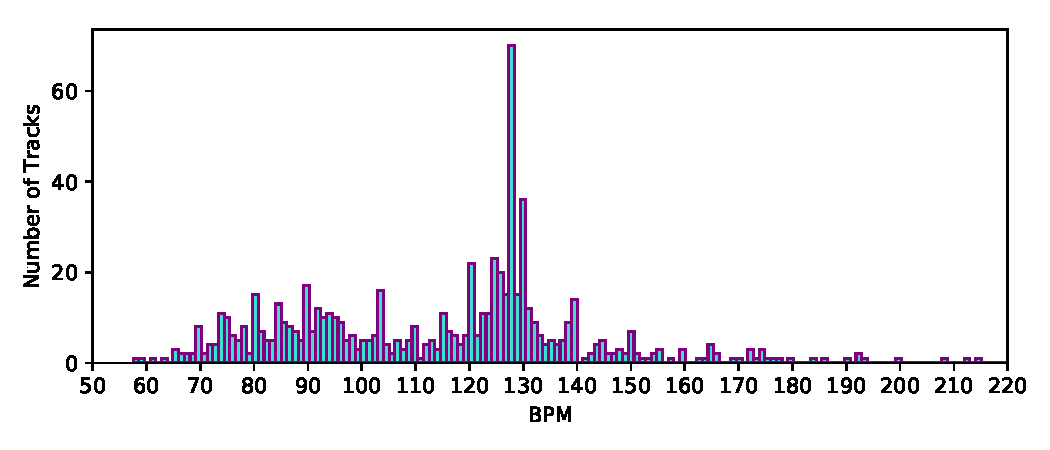
\includegraphics[width=\columnwidth]{figs/BPM_distribution.pdf}}
    \caption{Tempo distribution of the tracks in the \setName~set.}
    \label{fig:BPM_dist}
\end{figure}

\begin{figure}
    \centerline{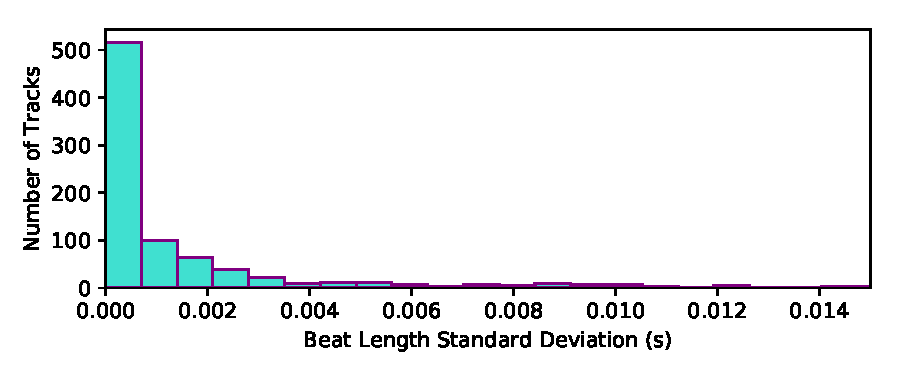
\includegraphics[width=\columnwidth]{figs/BPM_std.pdf}}
    \caption{Standard deviation of the tempo distribution in the \setName~set.}
    \label{fig:BPM_std}
\end{figure}

In terms of segment statistics, we show data based on certain attributes described in a MIREX meta-analysis of the segmentation task~\cite{Smith2013}.
In Figure~\ref{fig:segment_count} we plot track-level histograms for the number of segments, and the number of unique segments (i.e., those with the same associated label).
Both distributions seem to be unimodal and centered around 10 and 11 for the number of segments per tracks, and around 6 and 7 for the number of unique labels per track.
This differs from the number of unique segments in The Beatles dataset, which is centered around 4 per track~\cite{Nieto2014}.

\begin{figure}
    \centerline{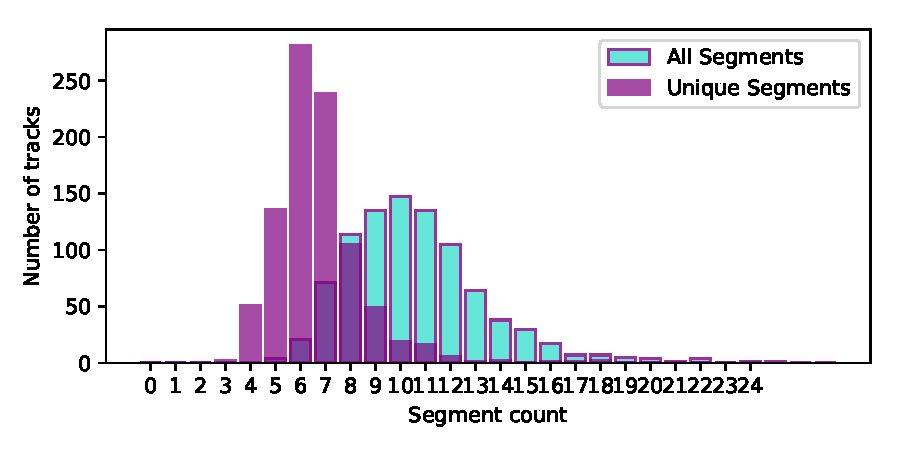
\includegraphics[width=\columnwidth]{figs/segment_label_count.pdf}}
    \caption{Number of segments per track, based on their segment labels.}
    \label{fig:segment_count}
\end{figure}

Figure~\ref{fig:seglabel_dist} shows the frequency in which the most common segment labels appear in the set.
The labels ``chorus'' and ``verse'' dominate the distribution, as these functional parts are common in western popular music.
The plot also shows potentially repeated labels like ``inst'' and ``instrumental.''
A further inter-song analysis of the labels might be necessary to potentially merge certain labels and thus unify the vocabulary of the set.

\begin{figure}
    \centerline{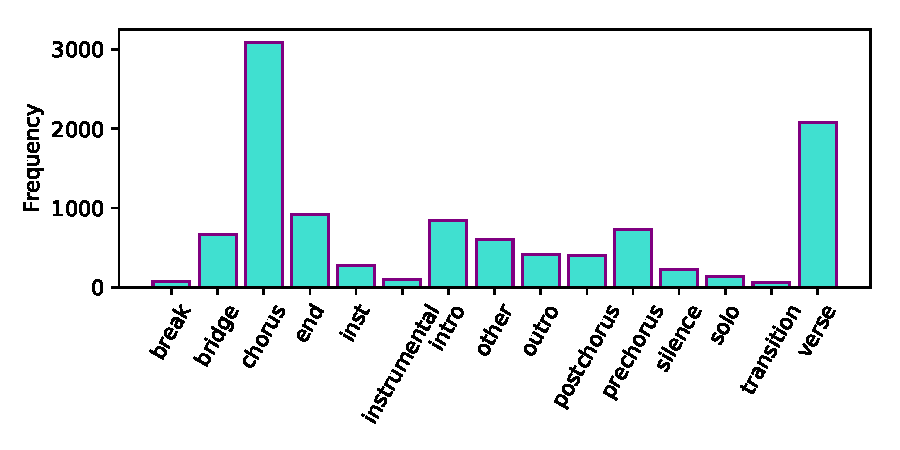
\includegraphics[width=\columnwidth]{figs/SegmentLabels_distribution.pdf}}
    \caption{Most common segment labels.}
    \label{fig:seglabel_dist}
\end{figure}

We plot in Figure~\ref{fig:seglen_dist} the distribution of the segment lengths, in seconds, across the entire dataset.
It might be interesting to discuss the peak at 15 seconds.
As we showed in Figure~\ref{fig:BPM_dist}, there is a majority of tracks at 128 BPM, which makes 15 seconds a segment of exactly 32 beats.
This, in the common 4/4 time signature, would result in 8 bars per each 15-second segment in that tempo, and 8 bars are rather usual in electronic dance music~\cite{Moelants2008}.

\begin{figure}
    \centerline{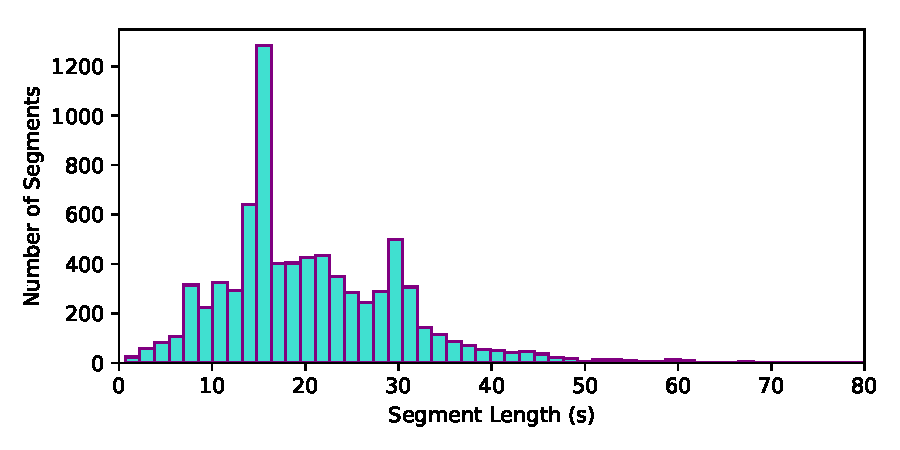
\includegraphics[width=\columnwidth]{figs/SegmentLength_distribution.pdf}}
    \caption{Segment length distribution.}
    \label{fig:seglen_dist}
\end{figure}

Finally, and thanks to having access to the annotated downbeats, we show in Figure~\ref{fig:downbeat_segment} the number of segments starting at a specific beat within a given bar.
We can see that the vast majority of segments (81.1\%) start in a downbeat.
Interestingly, several segments (10\%) start in position 4, thus showing that 1-beat count-ins are more common than other types of count-ins on this dataset.

\begin{figure}
    \centerline{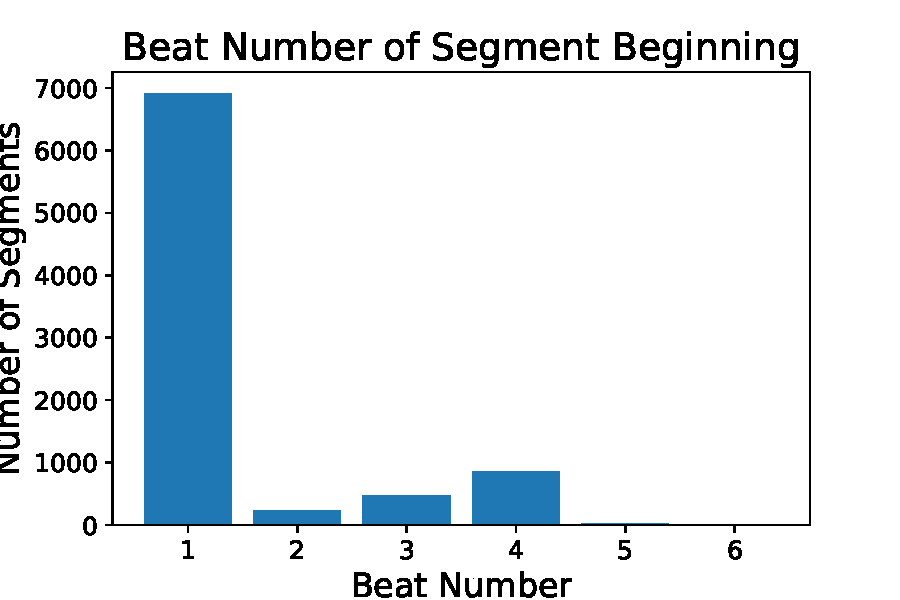
\includegraphics[width=\columnwidth]{figs/Downbeat_Segment_Alignment.pdf}}
    \caption{Number of segments based on their starting beat position within a bar.}
    \label{fig:downbeat_segment}
\end{figure}

\section{Results}\label{sec:results}

\subsection{Beat Results}

In order to establish performance baselines over the dataset for the task of beat-tracking. We have evaluated a number of openly available beat
tracking algorithms on the dataset \cite{Ellis2007, Krebs2015, Korzeniowski2014, Bock2011}. Each of these algorithms can be found in either the
Madmom \cite{Bock2016b} or Librosa \cite{Mcfee2015a} python libraries. This allows a comparison between datasets for which these algorithms have been previously evaluated,
with respect to their affect on these algorithm's performance. The results are also provided with the dataset in CSV format. This is intendended
as a convenience for any future work that wishes to evaluate novel algorithms against these benchmarks.

The beat tracking results for the aforementioned algorithms are displayed in Figure~\ref{fig:beat_results}. There they are evaluated across two metrics,
F-Measure, and Max~F-Measure, where the latter refers to the maximum F-Measure obtained per track when evaluated across double and half-time metrical variations
in the annotated beats provided with this dataset. For half-time metrical variations, both the downbeat and offbeat alignments were tested for a maximum F-Measure
value. While \cite{Ellis2007} is the most computationally efficient of the algorithms, we see clear gains in the later methods developed. It can be seen that with 
this dataset, both \cite{Ellis2007} and the ``BeatDetector'' algorithm from \cite{Bock2011} when using  and REF have a significant number of double-half time errors, compared to REFS.
Unlike the ``BeatTracker'' algorithm in \cite{Bock2011}, the ``BeatDetector'' algorithm assumes constant tempo.

\begin{figure}
    \centerline{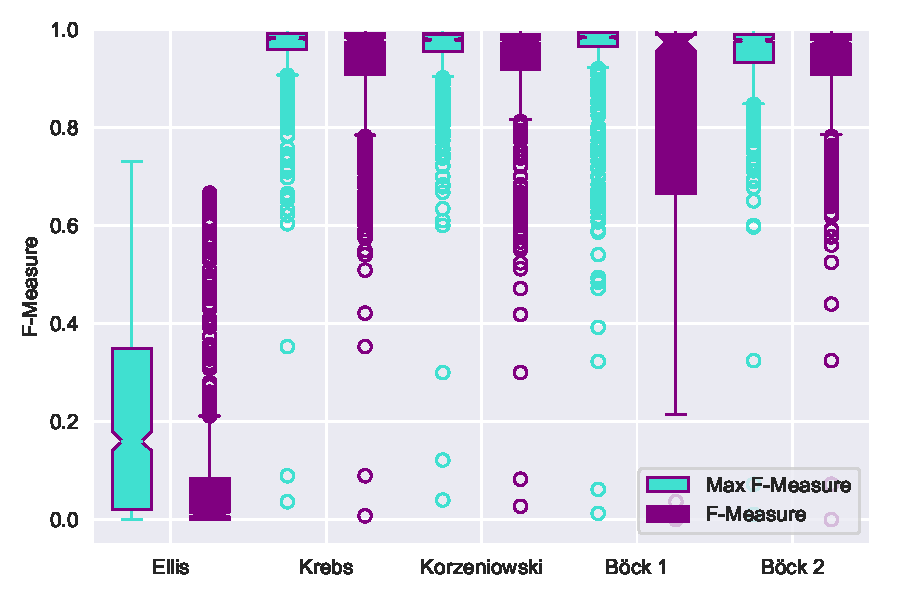
\includegraphics[width=\columnwidth]{figs/2019_04_09_19_15_00_Beat_TrackiMax_F-Measure.pdf}}
    \caption{Beat tracking performance over the \setName~set, for the algorithms Ellis \cite{Ellis2007}, Krebs \cite{Krebs2015}, Korzeniowski \cite{Korzeniowski2014}, B{\"o}ck 1 - the ``BeatDetector'' technique from \cite{Bock2011}, and B{\"o}ck 1 - the ``BeatTracker'' technique from \cite{Bock2011}.}
    \label{fig:beat_results}
\end{figure}

\subsection{Downbeat Results}

Unfortunately the availability of open source downbeat estimation libraries is limited. In order to provide a baseline for downbeat detection performance
with the \setName~set specifically, results have been evaluated with the downbeat detection algorithms available in \cite{Bock2016b}. Two algorithms were
evaluated including the method proposed in \cite{Bock2016a}, and the dynamic Bayesian bar tracking processor using the input from the RNN bar processor activation
function - all of which is available within the Madmom package \cite{Bock2016b}. The results can be seen in Figure~\ref{fig:downbeat_results}. For the method in \cite{Bock2016a}, the annotated beats are provided from which
to estimate the downbeats. The significant improvement in performance obtained by this algorithm over that with the estimated beat positions highlights the importance
of reliable beat tracking for downbeat estimation performance, and the interdependence between the beat tracking and downbeat estimation tasks.

\begin{figure}
    \centerline{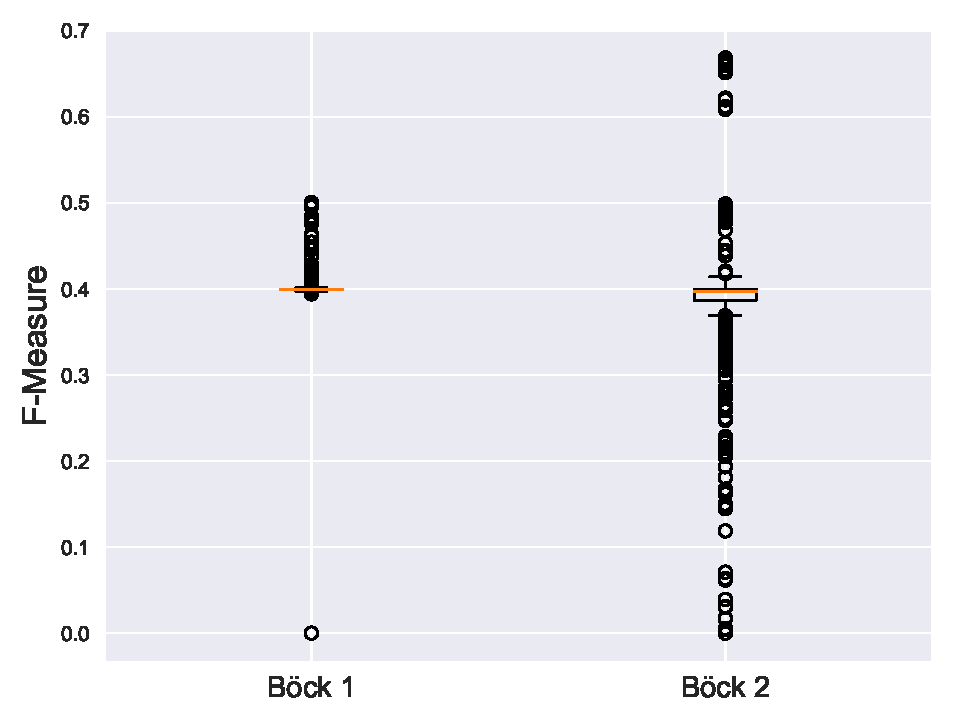
\includegraphics[width=\columnwidth]{figs/2019_04_09_10_27_35_Downbeat_Re_F-Measure.pdf}}
    \caption{Downbeat tracking performance over the \setName~set, for the algorithms B{\"o}ck 1 \cite{Bock2016a} and B{\"o}ck 2 - a dynamic Bayesian network provided within the Madmom package \cite{Bock2016b}.}
    \label{fig:downbeat_results}
\end{figure}

\subsection{Segmentation Results}

There are several open source structural segmentation algorithms available in the Music Structure Analysis Framework (MSAF)~\cite{Nieto2016}.
We run the most performing ones on the \setName~set.
These are the Structural Features~\cite{Serra2014} to identify boundaries, and the 2D-Fourier Magnitude Coefficients (2D-FMC)~\cite{Nieto2014} to label the segments based on their acoustic similarity.
We use \texttt{mir\_eval}~\cite{Raffel2014} to evaluate these algorithms, and report the F-measures of the most common metrics of Hit Rate at 0.5 and 3 seconds for boundary retrieval, and the Pairwise Frame Clustering and Entropy Scores for the labeling process.
These algorithms can use beat-synchronized features, and we ran each algorithm twice: once with estimated features using Librosa, and the other by using the actual annotated beats.
Song-level results for these two different runs are available as CSV files in the dataset repository disclosed above.

In Figure~\ref{fig:segment_results} all segmentation results are shown.
The results in turquoise boxplots display the metrics of the algorithms when running on estimated beat-synchronized features, while the purple boxplots show those using annotated beats instead.
Given how related boundary retrieval is with respect to beat placement, it is not unexpected to see a significant improvement in the boundary metrics (Hit Rates) when using annotated beats compared to those using estimated ones.
This illustrates the relevant room for improvement in terms of beat tracking (at least that contained in the Librosa package).
On the other hand, it is worth noting that the label results do not seem to depend as much on the quality of the beats in order to produce their outcomes, as the two different runs yield similar results.
As mentioned in Section~\ref{sub:structsegm}, structural segmentation is a challenging task especially due to ambiguity, subjectivity, and hierarchy, and this is reflected in the overall results, which have significant room for improvement.

\begin{figure}
    \centerline{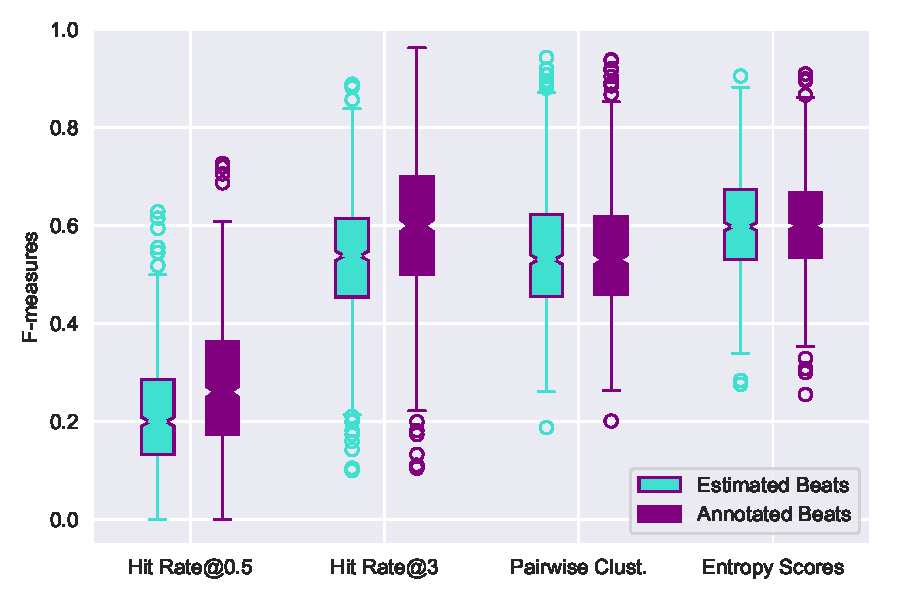
\includegraphics[width=1.1\columnwidth]{figs/segment_results.pdf}}
    \caption{Segmentation results over the \setName~set, using Structural Features for boundaries and 2D-FMC for the labeling process.}
    \label{fig:segment_results}
\end{figure}

\section{Conclusions}\label{sec:conclusions}

We presented the \setName~set, the largest dataset in terms of human annotations containing the following three types of music information: beats, downbeats, and function structural segments.

TODO: Potential of combined data + large amounts of annotations.

% For bibtex users:
\bibliography{ISMIRtemplate,beat_data_refs}

\end{document}
